\subsection*{Results and Discussion}

\begin{table}[H]
    \centering
    \begin{tabular}{|c|c|c|}
    \hline
    R & Loss & RelFit \\
    \hline
    1 & 1 & 77.589 \\
    \hline
    2 & 0.0975 & 96.497 \\
    \hline
    3 & 0.0065 & 98.891 \\
    \hline
    4 & 0.0045 & 98.936 \\
    \hline
    5 & 0.0028 & 98.967 \\
    \hline
    \end{tabular}
    \caption{Loss relative to loss for $R=1$ and RelFit for $R=1,2,3,4,5$ for best model of 20 runs for each $R$.}
    \label{tab:rank_choice}
\end{table}

\gaute{discuss discovered rank}

\gaute{discuss uniqueness results (all equal, not for r=4 though)}

\begin{figure}[H]
    \centering
    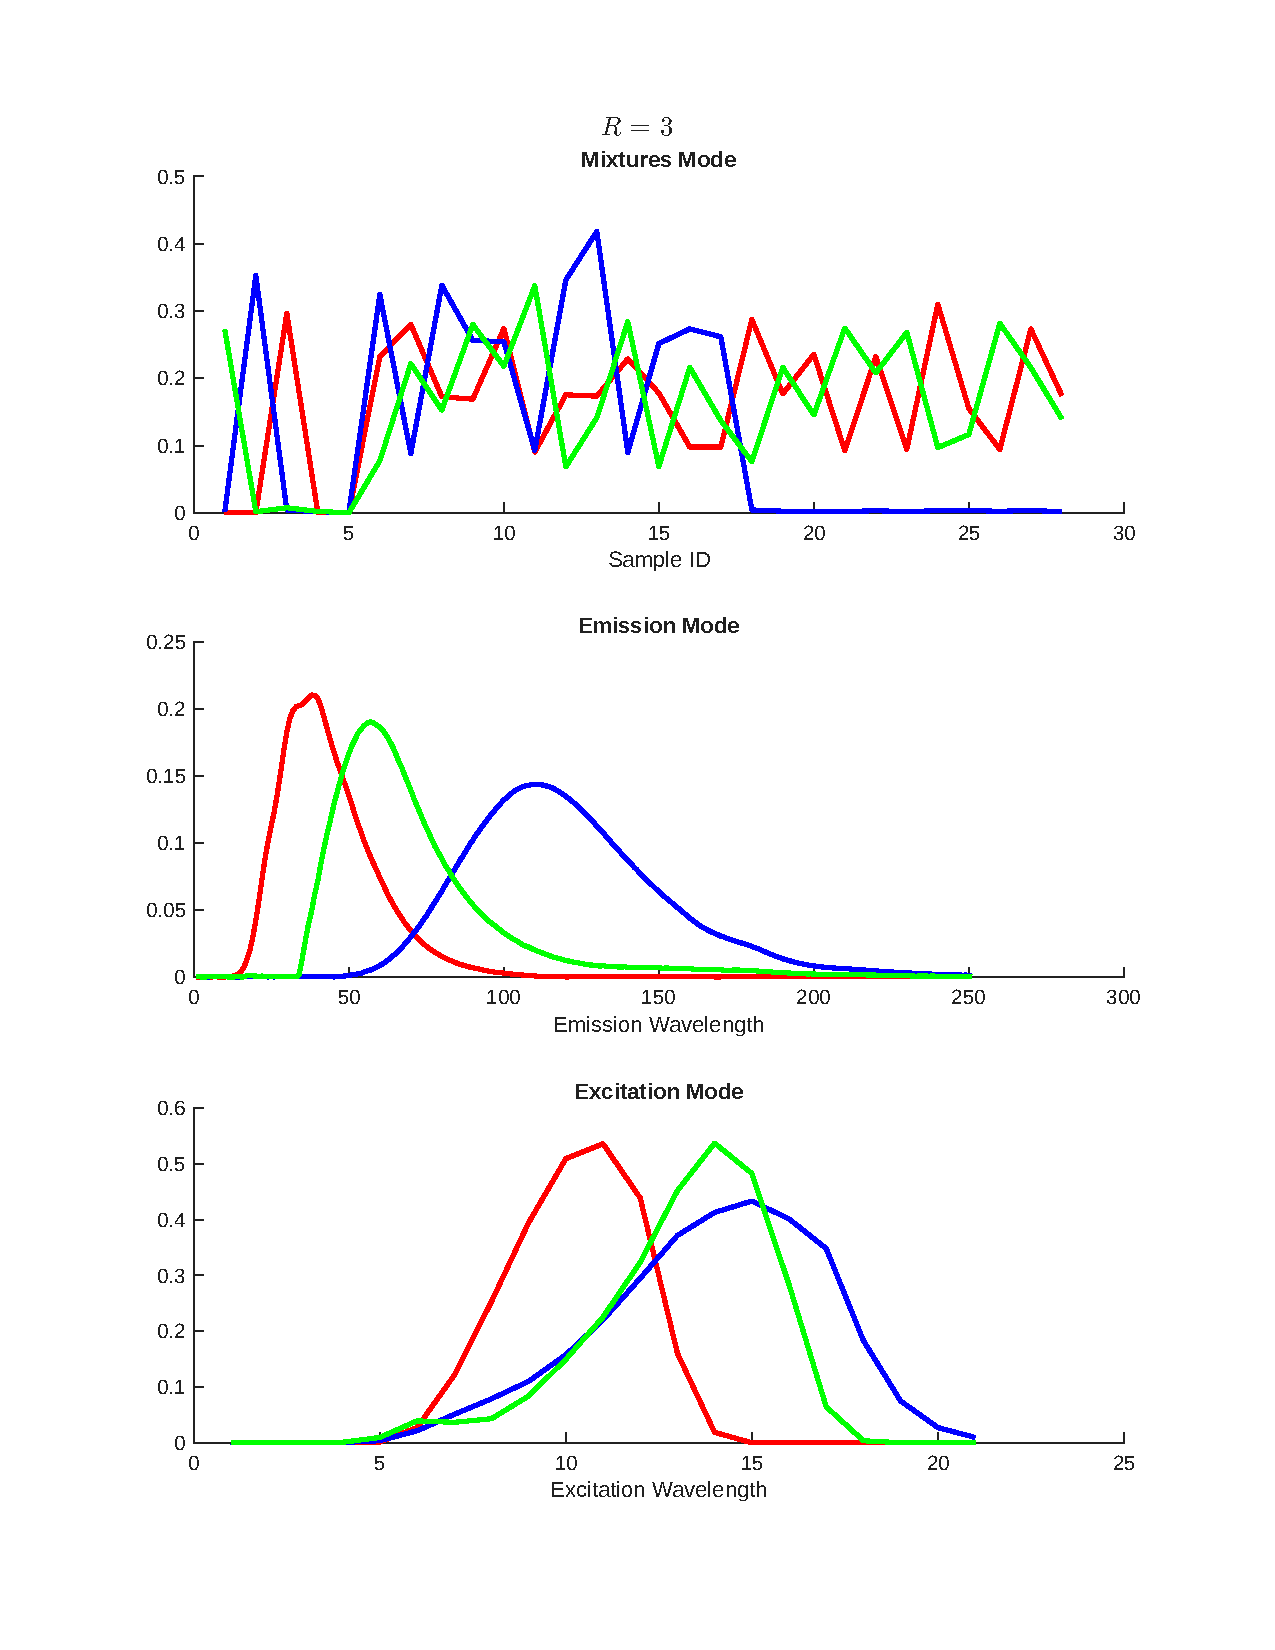
\includegraphics[trim = 2cm 2.5cm 2cm 1.9cm, clip, width=0.46\linewidth]{figures/factors_rank3.pdf}
    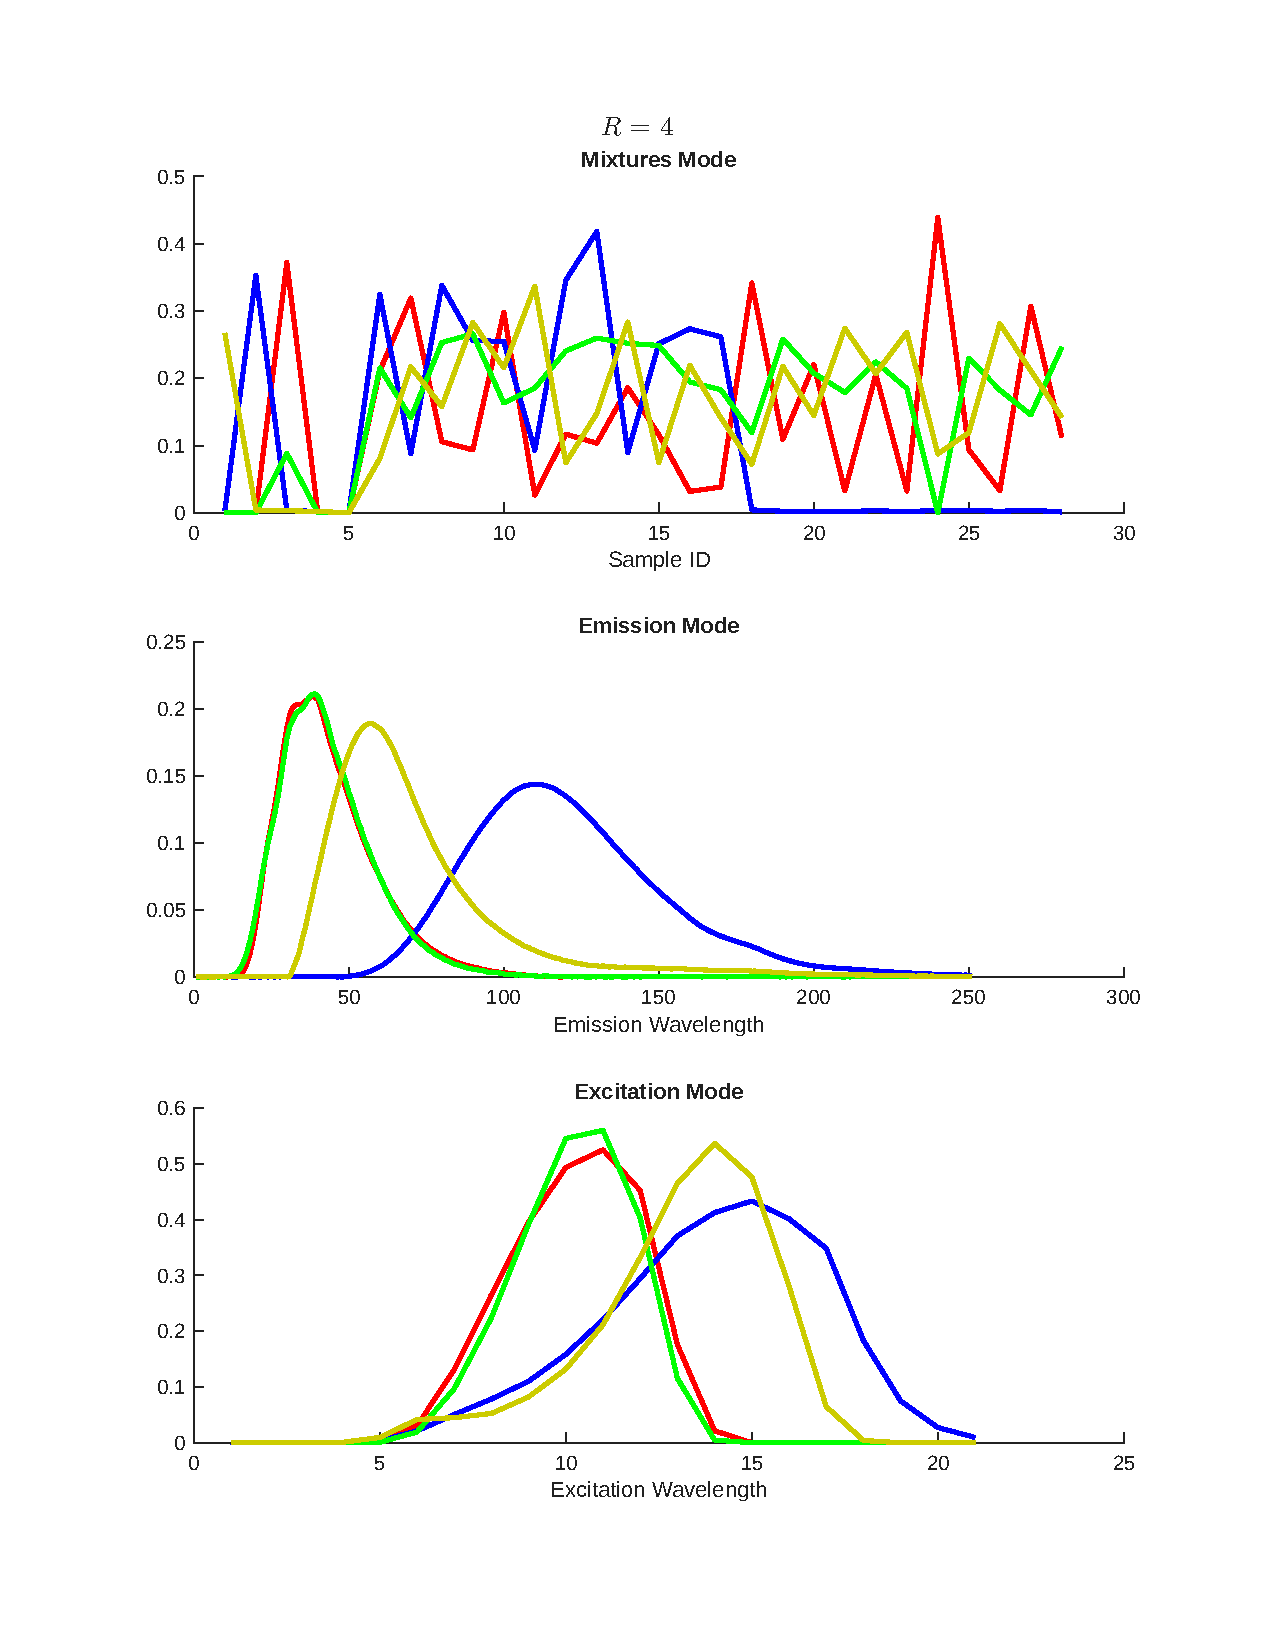
\includegraphics[trim = 2cm 2.5cm 2cm 1.9cm, clip, width=0.46\linewidth]{figures/factors_rank4.pdf}
    \caption{\gaute{note that these factors are normalized}}
    \label{fig:plot_factors}
\end{figure}

\gaute{Explain discovered factors}
